\documentclass{article}

% ─────────────────────────── PACKAGES ────────────────────────────
\usepackage{times}
\usepackage{geometry}
\geometry{a4paper,left=0.6cm,right=0.7cm,top=1cm,bottom=1cm,columnsep=0.8cm}

\usepackage{fontawesome}
\usepackage[hidelinks]{hyperref}
\usepackage{paracol}
\usepackage{tikz}
\usepackage{tabularx}
\usepackage{xcolor}
\usepackage{enumitem}


\definecolor{maincolor}{HTML}{ffffff}
\definecolor{seccolor}{HTML}{0b1f3b}
\definecolor{gray}{HTML}{8c94a9}
\definecolor{sidetext}{HTML}{59cee5}
\definecolor{Green}{HTML}{2caf00}
\definecolor{lightgray}{HTML}{D3D3D3}
%\definecolor{maincolor}{HTML}{2AAEE7}

\newcolumntype{Y}{>{\RaggedRight\arraybackslash}X}
\setlist[itemize]{itemsep=-2pt,topsep=0pt,leftmargin=*}
\renewcommand{\labelitemi}{\textcolor{black}{\footnotesize$\bullet$}}
%
\setlength{\parindent}{0pt}

% titre de section
\newcommand{\cvsection}[1]{%
  \par\bigskip
  \begin{tabular}{@{}p{\linewidth}}
  \textbf{\Large #1}\\[3pt]\hline
  \end{tabular}\medskip}

\newcommand*{\ClipSep}{0.4cm}

\setlength{\columnseprule}{0.4pt}        % épaisseur du trait
\setlength{\columnsep}{0.8cm}            % (facultatif : rappel de l’écart)
\def\columnseprulecolor{\color{lightgray}}% couleur du trait
% ─────────────────────────── DOCUMENT ────────────────────────────
\begin{document}\pagestyle{empty}
\columnratio{0.7}\begin{paracol}{2}

%%%%%%%%%%%%%%%%%%%%%%%%%%%%%%%%%%%%%%%%%%%%%%%%%%%%%%%%%%%%%%%%%%%
% Colonne gauche (70 %)
%%%%%%%%%%%%%%%%%%%%%%%%%%%%%%%%%%%%%%%%%%%%%%%%%%%%%%%%%%%%%%%%%%%

{\LARGE\textbf{Judikael Mourouvin}}

\bigskip
{\color{sidetext}\Large\textbf{Technicien support \& marketing digital}}

\medskip
\begin{tabular}{@{}cp{0.4\linewidth}cp{0.4\linewidth}}
  \color{sidetext}\faEnvelope & \href{mailto:jkmou971@gmail.com}{jkmou971@gmail.com} &
  \color{sidetext}\faMapMarker & Route de COCOYER\;97190 GOSIER\\[6pt]
  \color{sidetext}\faPhone & \href{tel:+590 0690 91 14 48}{+590 0690 91 14 48} &
  \color{sidetext}\faLinkedin & \href{}{}
\end{tabular}

\cvsection{EXPERIENCE}

\colorbox{maincolor}{%
  \begin{minipage}{\linewidth}
    \textbf{Alternant en Marketing Digital} \\ Mairie du Gosier – DSI \\ 2023-2024
    \begin{itemize}
      \item Piloté des projets numériques et assuré leur déploiement dans les délais impartis. \item Analysé les besoins utilisateurs, déployé des solutions adaptées puis assuré support et formations. \item Contribué à la stratégie de marketing digital pour accroître la visibilité de la collectivité.
    \end{itemize}
  \end{minipage}}

\vspace{3mm}


\colorbox{maincolor}{%
  \begin{minipage}{\linewidth}
    \textbf{Animateur de la zone informatique} \\ Pôle Emploi, Gosier \\ 2022-2023
    \begin{itemize}
      \item Assuré l’assistance et le support technique quotidiens auprès des demandeurs d’emploi. \item Configuré et maintenu les postes de travail pour garantir une disponibilité optimale. \item Diagnostiqué et résolu les incidents matériels et logiciels afin de réduire les interruptions de service.
    \end{itemize}
  \end{minipage}}

\vspace{3mm}


\colorbox{maincolor}{%
  \begin{minipage}{\linewidth}
    \textbf{Stagiaire Informaticien} \\ NUMERIKA, Baie-Mahault \\ 2020-2021
    \begin{itemize}
      \item Installé, configuré et maintenu les équipements informatiques du parc. \item Apporté un support de proximité aux utilisateurs et documenté les interventions.
    \end{itemize}
  \end{minipage}}      %← généré dynamiquement (blocs colorbox)

\cvsection{EDUCATION}

    \begin{tabularx}{\linewidth}{@{}c >{\RaggedRight\arraybackslash}X@{}}
    \textcolor{sidetext}{\faGraduationCap} &
    \textbf{Bachelor Marketing Digital} \\
    & CFA IUTS \\
    & \textit{2023-2024} \\
    \end{tabularx}
    \begin{itemize}[leftmargin=*]
  \item Stratégies de référencement, gestion de campagne web et réseaux sociaux.
  \item Analyse de données marketing et optimisation de la performance digitale.
\end{itemize}
\vspace{3mm}

    \begin{tabularx}{\linewidth}{@{}c >{\RaggedRight\arraybackslash}X@{}}
    \textcolor{sidetext}{\faGraduationCap} &
    \textbf{BTS Système Numérique option Informatique et Réseaux} \\
    & Lycée de Chevalier Saint Georges, Abymes \\
    & \textit{2019-2021} \\
    \end{tabularx}
    \begin{itemize}[leftmargin=*]
  \item Architecture et administration de réseaux locaux et distants.
  \item Maintenance matérielle et logicielle, support utilisateur et cybersécurité.
\end{itemize}          %← idem



%%%%%%%%%%%%%%%%%%%%%%%%%%%%%%%%%%%%%%%%%%%%%%%%%%%%%%%%%%%%%%%%%%%
% Colonne droite (30 %)
%%%%%%%%%%%%%%%%%%%%%%%%%%%%%%%%%%%%%%%%%%%%%%%%%%%%%%%%%%%%%%%%%%%
\switchcolumn
\centering
\begin{tikzpicture}
  \clip (0,0) circle (1.5cm) node[anchor=center]
        {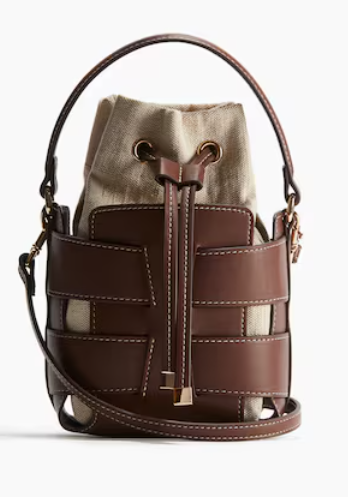
\includegraphics[width=3cm]{5eb2294ae81144b08f3a051b0bdb6a1c.png}};
\end{tikzpicture}


\cvsection{SUMMARY}
Passionné par l’informatique et le marketing digital, j’ai développé de solides compétences en configuration de postes, maintenance et diagnostic d’incidents. Mon alternance à la DSI de la Mairie du Gosier m’a permis de gérer des projets numériques et de former des utilisateurs. Aujourd’hui, je souhaite poursuivre à temps plein afin de mettre ma rigueur et mon sens du service au profit de nouveaux défis. Mon objectif : contribuer efficacement à la réussite de vos projets digitaux et informatiques.

\cvsection{SKILLS}
\begin{itemize}[leftmargin=*]
\item Administration
\item Maintenance
\item Réseaux
\item Support
\item Assistance
\item Marketing
\item Digital\end{itemize}

\cvsection{LANGUAGES}
\begin{itemize}[leftmargin=*]
\item English - \textcolor{gray}{}
\item Espagnol - \textcolor{gray}{}\end{itemize}

\cvsection{INTERESTS}
\begin{itemize}[leftmargin=*]
\item Lectur
\item Sports
\item Musique
\item Voyage
\end{itemize}

\end{paracol}
\end{document}
